\documentclass[12pt,letterpaper,margin=1in]{article}
% \documentclass[twocolumn]{aastex61}

% to-do list
% ----------
% - Fit summary in the first page.

% style notes
% -----------
% - This file generates by Makefile; don't be typing ``pdflatex'' or some bullshit.
% - Line break between sentences to make the git diffs readable.
% - Use \, as a multiply operator.
% - Reserve () for function arguments; use [] or {} for outer shit.
% - Use \sectionname not Section, \figname not Figure, \documentname not Article or Paper or paper.
% - Use "comoving" instead of "co-moving".
% - Use "phase space" not "phase-space", "phase-space coordinates" not "phase space coordinates".
% - Write elements as \elem{X}.

% packages
\usepackage[letterpaper,margin=1in]{geometry}

\usepackage{setspace}
\doublespacing
\usepackage{lineno}
\linenumbers
\usepackage{microtype}  % ALWAYS!
\usepackage{amsmath,amssymb}
\usepackage[sort&compress,super]{natbib}
\usepackage{graphicx}
\graphicspath{{figures/}}
\usepackage{aas_macros}
\usepackage{hyperref}
\hypersetup{backref,breaklinks,colorlinks,citecolor=blue}
\usepackage{mathptmx}
\usepackage{threeparttable}

% per section figure counting
\usepackage{chngcntr}
\counterwithin{figure}{section}

%\setcitestyle{super}
\citestyle{nature}
\bibliographystyle{naturemag}

% define macros for text
\newcommand{\project}[1]{\textsl{#1}}
\newcommand{\acronym}[1]{{\small{#1}}}
\newcommand{\gaia}{\project{Gaia}}
\newcommand{\rave}{\project{\acronym{RAVE}}}
\newcommand{\apogee}{\project{\acronym{APOGEE}}}
\newcommand{\tmass}{\project{\acronym{2MASS}}}
\newcommand{\documentname}{Article}
\newcommand{\sectionname}{Section}
\newcommand{\figname}{Figure}
\newcommand{\eqname}{Equation}
\newcommand{\dr}{\acronym{DR1}}
\newcommand{\tgas}{\acronym{TGAS}}
\newcommand{\etal}{\textit{et al}.}
\newcommand*\elem[1]{\ensuremath{\mathrm{#1}}}
\newcommand*\elemH[1]{\ensuremath{[\mathrm{#1}/\elem{H}]}}
\newcommand*\teff{\ensuremath{T_\mathrm{eff}}}
\newcommand*\logg{\ensuremath{\log{g}}}
\newcommand*{\feh}{\ensuremath{\elemH{Fe}}}
\newcommand{\sunanalog}{\text{Krios}}
\newcommand{\bizarreone}{\text{Kronos}}
\newcommand{\Tcondens}{\ensuremath{T_C}}
\newcommand{\mearth}{\ensuremath{M_\oplus}}
\newcommand{\mjupiter}{\ensuremath{M_\mathrm{Jup}}}

% define macros for math
\newcommand{\given}{\,|\,}
\newcommand{\normal}{{\mathcal{N}}}
\newcommand{\dd}{\mathrm{d}}
\newcommand{\transp}[1]{{#1}^{\!\mathsf{T}}}
\newcommand{\inv}[1]{{#1}^{-1}}
\newcommand{\bs}[1]{\boldsymbol{#1}}
\newcommand{\vperp}{\bs{v}^\perp}
\newcommand{\propm}{\bs{\mu}}
\newcommand{\mat}[1]{\mathbf{#1}}
\renewcommand{\vec}[1]{\bs{#1}}
\newcommand{\kms}{\ensuremath{\rm km~s^{-1}}}
\newcommand{\msun}{\ensuremath{{\mathrm M}_\odot}}
\newcommand{\pc}{{\rm pc}}
\newcommand{\data}{\mathrm{data}}
\newcommand{\snr}{[S/N]_\varpi}
\newcommand{\eye}{\mathbb{I}}
\newcommand{\absdvtan}{\ensuremath{|\Delta\vec v_\mathrm{t}|}}
\newcommand{\estimates}{\ensuremath{\{\hat{\varpi_i},\hat{\mu_{\alpha,i}},\hat{\mu_{\delta,i}},\hat{v_{r,i}}\}}}

\newcommand{\todo}[1]{{\color{red}TODO: #1}}

\renewcommand\tablename{Table}




% Titles:
% - 90 characters (including spaces)
% - do not normally include numbers, acronyms, abbreviations or punctuation
% - They should include sufficient detail for indexing purposes but be general
%   enough for readers outside the field to appreciate what the paper is about.
\title{
\vspace{-2cm}
  Kronos \& Krios: Evidence for accretion of rocky planets in a comoving pair of sun-like stars
  \vspace{-0.5cm}
}

\author{
  Semyeong Oh$^{1,*}$,\,
  Adrian M. Price-Whelan$^{1}$,\,
  John M. Brewer$^{2}$,\,\\
  David W. Hogg$^{3,4,5,6}$,\,
  David N. Spergel$^{1,3}$,\,
  Justin Myles$^{2}$
}
\date{\small\today}

\begin{document}\sloppy\sloppypar\raggedbottom\frenchspacing % trust me
\maketitle

% affiliations
\vspace{-1cm}
{\small\noindent
  $^1$Department of Astrophysical Sciences, Princeton University, 4 Ivy Lane, Princeton, NJ 08544, USA \\
  $^2$Department of Astronomy, Yale University, 260 Whitney Ave, New Haven, CT 06511, USA \\
  $^3$Center for Computational Astrophysics, Flatiron Institute, 162 Fifth Ave, New York, NY 10010, USA \\
  $^4$Center for Data Science, New York University, 60 Fifth Ave, New York, NY 10011, USA \\
  $^5$Center for Cosmology and Particle Physics, Department of Physics, New York University, 726 Broadway, New York, NY 10003, USA \\
  $^6$Max-Planck-Institut f\"ur Astronomie, K\"onigstuhl 17, D-69117 Heidelberg \\
  $^*$To whom correspondence should be addressed: \texttt{semyeong@astro.princeton.edu}
}

%% \author{Keith A. Hawkins}
%% \affil{Department of Astronomy, Columbia University, 550 W 120th St, New York, NY 10027, USA}

%% \author{Nathan W. C. Leigh}
%% \affil{Department of Astrophysics, American Museum of Natural History, Central Park West and 79th St, New York, NY 10024, USA}



% ------------------------
% nature summary paragraph
% ------------------------
% - a fully referenced paragraph, ideally of about 200 words, but certainly no
%   more than 300 words, aimed at readers in other disciplines.
% - This paragraph starts with a 2-3 sentence basic introduction to the field;
%   followed by a one-sentence statement of the main conclusions starting 'Here
%   we show' or equivalent phrase; and finally, 2-3 sentences putting the main
%   findings into general context so it is clear how the results described in
%   the paper have moved the field forwards.
% - annotated example: https://www.nature.com/nature/authors/gta/2c_Summary_para.pdf
% ------------------------
\section{Summary}
{\bf \noindent
  Stars that are born together are expected to have the same chemical
  compositions initially.
  Detailed chemical abundance studies of stars in wide binaries indeed reveal
  little to no abundance differences in most
  cases\citep{Gratton:2001aa,Desidera:2004aa}.
  However, the formation and evolution of different planetary systems around
  each star in a wide binary may eventually lead to differences in the chemical
  abundances of the component stars' radiative and convective
  layers\cite{Pinsonneault:2001aa,Chambers:2010aa}.
  Wide binary systems of two twin-like stars are particularly useful since such
  chemical signature may be more easily detectable as abundance differences,
  free from dependences on stellar parameters or confusion with Galactic
  chemical evolution.
  A handful of wide binaries that show small differences ($0.03$--$0.1$~dex)
  in their surface chemical abundances have been reported so far
  \cite{Mack:2014aa,Mack:2016aa,Saffe:2015aa,Teske:2013aa,
    Teske:2015aa,Teske:2016aa,Teske:2016ab,Biazzo:2015aa,Ramirez:2015aa},
  however, a conclusive example of planetary accretion has not yet been found.
  %
  Here we report the discovery of a comoving pair of bright, sun-like
  stars---HD~240430 and HD~240429, hereafter ``\bizarreone'' and
  ``\sunanalog''--- with significant differences ($\approx 0.2$~dex) in their
  chemical abundances that strongly suggest accretion of a massive rocky
  planetary system in one of the stars within the last billion years.
  The more metal-rich of the two, \bizarreone, shows an enhancement of refractory
  elements by $\approx 0.2$~dex and a small enhancement ($\lesssim 0.11$~dex) of
  (moderately) volatile elements.
  The two stars also show high \elem{Li} abundance given their age of $\sim 4$ Gyr,
  as inferred from their stellar parameters.
  We suggest that the star \bizarreone\ accreted
  $\approx 15$~\mearth\ of rocky material, selectively enhancing the
  refractory elements in its surface and convective envelope.
  The other star, \sunanalog, may also have had a similar accretion
  event given its high surface \elem{Li} abundance but of much smaller amount
  ($\approx 4$~\mearth).
  This pair of stars provides evidence that dynamical accretion of rocky planets
  does happen during the main-sequence lifetime of sun-like stars.
}

\section{Main Text}

\begin{figure}[htpb]
  \centering
  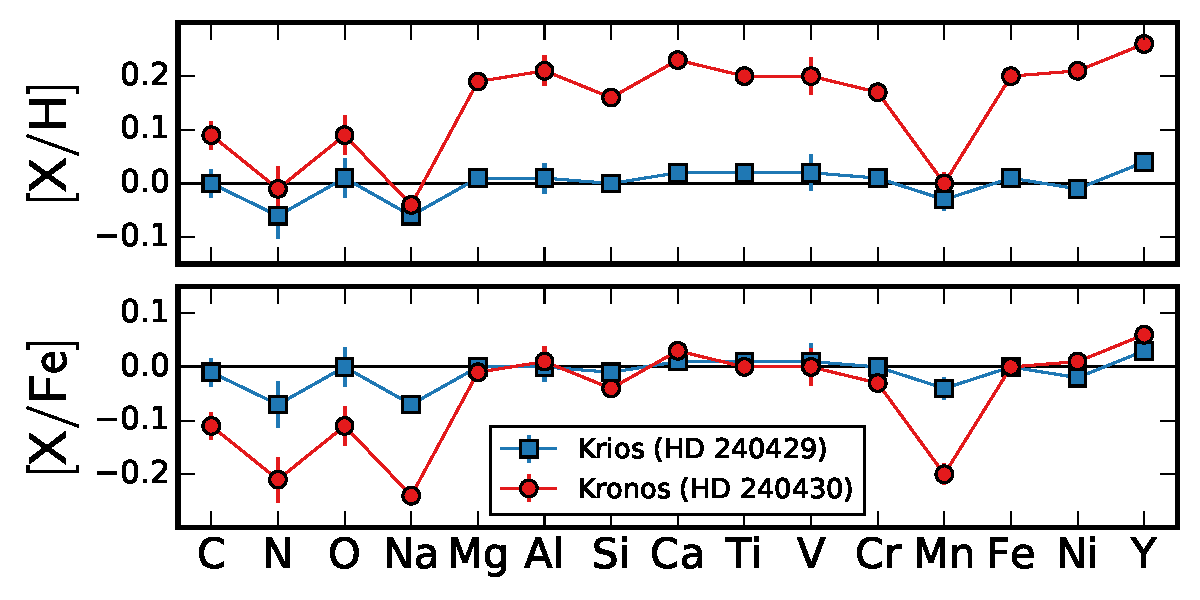
\includegraphics[width=0.9\linewidth]{abundances.pdf}
  \caption{Abundances of the comoving pair,
    \bizarreone\ (red circles) and \sunanalog\ (blue squares).
    Lines are drawn for each star only to guide the eye.
    \bizarreone\ is enhanced in \elem{Fe} by $\approx 0.2$~dex relative to
    \sunanalog\ along with \elem{Mg}, \elem{Al}, \elem{Si}, \elem{Ca},
    \elem{Ti}, \elem{V}, \elem{Cr}, \elem{Ni}, \elem{Y} yet much less in
    \elem{C}, \elem{N}, \elem{O}, \elem{Na}, and \elem{Mn}.
    \label{fig:abundances}
  }
\end{figure}

\begin{table*}[htpb]
  \centering
  \begin{threeparttable}
  \caption{Astrometric and spectroscopic measurements of the pair\label{tab:t1}}
\begin{tabular}{ccccc}
\hline\hline
                        &                & \sunanalog\            & \bizarreone\           &               \\
Name                    & Units          & HD 240429              & HD 249439              & Uncertainties \\
\hline
Sp Type                 &                & G2                     & G0                     &               \\
R.A.\tnote{a}           & hh:mm:ss       & 23:51:55.21            & 23:52:09.42            &               \\
Dec.\tnote{a}           & dd:mm:ss       & 59:42:48.16            & 59:42:26.08            &               \\
2MASS $J$\tnote{a}      & mag            & $8.593 \pm 0.023$      & $8.415 \pm 0.026$      &               \\
$T_\mathrm{eff}$        & K              & 5878                   & 5803                   & 25            \\
$\log{g}$               &                & 4.43                   & 4.33                   & 0.028         \\
$v\sin{i}$              & \kms\          & 1.1                    & 2.5                    & 0.5           \\
$[\elem{Fe}/\elem{H}]$  &                & 0.01                   & 0.20                   & 0.010         \\
Age\tnote{b}            & Gyr            & $4.00_{-1.56}^{+1.51}$ & $4.28_{-1.03}^{+1.11}$ &               \\
$v_r$                   & \kms\          & $-21.2$                & $-21.2$                & 0.2           \\
$\varpi$\tnote{a}       & mas            & $9.35 \pm 0.24$        & $9.41 \pm 0.25$        &               \\
$\mu_\alpha^*$\tnote{a} & mas\,yr$^{-1}$ & $89.25 \pm 0.66$       & $89.41 \pm 0.69$       &               \\
$\mu_\delta$\tnote{a}   & mas\,yr$^{-1}$ & $-29.68 \pm 0.54$      & $-30.12 \pm 0.52$      &               \\
\hline
\multicolumn{5}{c}{$T_c < 1200$~K} \\
\hline
$A(\elem{Li})$\tnote{c} &                & $2.25$                 & $2.75$                 & 0.05          \\
$\elemH{C}$             &                & $0.00$                 & $0.09$                 & 0.026         \\
$\elemH{N}$             &                & $-0.06$                & $-0.01$                & 0.042         \\
$\elemH{O}$             &                & $0.01$                 & $0.09$                 & 0.036         \\
$\elemH{Na}$            &                & $-0.06$                & $-0.04$                & 0.014         \\
$\elemH{Mn}$            &                & $-0.03$                & $0.00$                 & 0.020         \\
\hline
\multicolumn{5}{c}{$T_c > 1200$~K} \\
\hline
$\elemH{Mg}$            &                & $0.01$                 & $0.19$                 & 0.012         \\
$\elemH{Al}$            &                & $0.01$                 & $0.21$                 & 0.028         \\
$\elemH{Si}$            &                & $0.00$                 & $0.16$                 & 0.008         \\
$\elemH{Ca}$            &                & $0.02$                 & $0.23$                 & 0.014         \\
$\elemH{Ti}$            &                & $0.02$                 & $0.20$                 & 0.012         \\
$\elemH{V}$             &                & $0.02$                 & $0.20$                 & 0.034         \\
$\elemH{Cr}$            &                & $0.01$                 & $0.17$                 & 0.014         \\
$\elemH{Fe}$            &                & $0.01$                 & $0.20$                 & 0.010         \\
$\elemH{Ni}$            &                & $-0.01$                & $0.21$                 & 0.014         \\
$\elemH{Y}$             &                & $0.04$                 & $0.26$                 & 0.030         \\
\hline
\end{tabular}
\begin{tablenotes}
\item [a] From \tgas.
\item [b] Derived in this work by isochrone fitting using the Yale-Yonsei model
  isochrones\cite{2013ApJ...776...87S}.
\item [c] Absolute abundances from Myles \etal\ (in prep.).
%\item All values are from \citet{2016ApJS..225...32B} unless otherwise noted.
\end{tablenotes}
\end{threeparttable}
\end{table*}


% general description of the pair and measurements
\sunanalog\ and \bizarreone\ were identified as a candidate comoving star pair
in our recent search\cite{2017AJ....153..257O} for comoving stars using the
proper motions and parallaxes from the {\it Tycho-Gaia Astrometric Solution}
catalog (hereafter \tgas), a component of the first data release of the
astrometric space mission \gaia\cite{2016A&A...595A...2G} (the astrometric
measurements are listed in \tablename~\ref{tab:t1}).
The pair has also been previously recognized as a visual double star system
in the Washington Double Star catalog\cite{2001AJ....122.3466M}.
The two stars have spectral types G0 and G2, both similar to the Sun (G2).
In a separate effort to study the detailed chemical abundances of potential
planet-hosting stars, high resolution ($R=\lambda/\Delta\lambda\approx 70000$),
high signal-to-noise ratio (typically $>200$ per pixel in continuum) spectra of
both stars for the wavelength range $5164$--$7799$~\AA\ were obtained using the
HIRES spectrograph on the Keck-I telescope\cite{2016ApJS..225...32B}.
The resulting measurements include elemental abundances for 15 chemical species
(C, N, O, Na, Mg, Al, Si, Ca, Ti, V, Cr, Mn, Fe, Ni, Y) as well as stellar
parameters and high precision ($\sigma\approx0.2$~\kms) radial velocities
(Table~\ref{tab:t1}).
The abundances are noted as \elemH{X}, defined as the log ratio of number
density of element \elem{X} to \elem{H} relative to the solar value
($\elemH{X} = \log_{10} ((n_X / n_H) / (n_X / n_H)_\odot)$).
Using the same spectra, lithium lines were modelled in Myles \etal, in prep.
For lithium, we use the absolute abundance defined as $A(\elem{Li}) = 12 +
\log_{10} (n_\elem{Li}/n_\elem{H})$.

% likely origin given its proximity in phase space
The projected separation between the pair is 1.9 arcmin\ ($\approx 0.01$~pc),
and the maximum-likelihood 3D separation is $\approx 0.6$~pc.
Although selected based only on their astrometry, the two stars
have identical radial velocities within uncertainties,
confirming that they are truly comoving (\sectionname~\ref{supp:dxdv}).
As the separation is smaller than the Jacobi radius (1.2~pc) in the solar
neighborhood for a 2~\msun\ binary system\cite{Jiang:2010aa}, \bizarreone\ and
\sunanalog\ are likely a coeval, bound wide-binary system.

% coevality based on stellar parameters
Their stellar parameters also indicate that they are coeval with an age of $\sim 4$~Gyr.
We use the distances (inferred from \gaia\ parallaxes), $V$-band magnitudes,
and $B-V$ colors to obtain bolometric luminosities of the two stars\cite{2003AJ....126..778V}.
We then combine the luminosities with effective temperature, \elemH{Fe}, and
\elemH{Si} in order to interpolate the age, mass, and radius of each star
using a grid of (Yale-Yonsei) model isochrones\cite{2013ApJ...776...87S}.
The best-fit isochrone ages of \bizarreone\ and \sunanalog\ are
$4.28_{-1.03}^{+1.11}$~Gyr and $4.00_{-1.56}^{+1.51}$~Gyr, respectively,
consistent with them being coeval (\figname~\ref{fig:yyisofitting}).

% metallicity and abundance difference
However, one of the stars, \bizarreone, is significantly more metal rich than
the other by 0.2~dex in \feh\ ($\approx 60\%$ in number density;
\figname~\ref{fig:abundances}).
Moreover, not all elements are equally enhanced: the abundances of \bizarreone\
show selective under-enhancement in \elem{C}, \elem{N}, \elem{O}, \elem{Na},
and \elem{Mn} relative to \elem{Fe} and other refractory elements.
As expected from their measured metallicity difference, the ratio of spectral
data and model between the two stars show significant residuals of almost all
metal line features, largely dominated by \elem{Fe}.
However, for absorption lines of elements that are not as enhanced in
\bizarreone\, the residuals are much smaller in amplitude demonstrating the
validity of the measured abundance differences (\figname~\ref{fig:spec1},
\ref{fig:spec2} and \ref{fig:spec_lithium}).

% novelty
The observed difference in metallicity and abundances is genuinely rare and
unexpected.
None of the other four twin-like ($\Delta T_\mathrm{eff} \lesssim 100$~K)
wide-binary pairs examined using spectra of similar quality and the same
consistent measurement procedure shows discrepancies in abundances between the
stars at this level\cite{2016ApJS..225...32B} (\figname~\ref{fig:deltaXH}).
The maximum metallicity difference observed in the other pairs is $\Delta\feh =
0.03$~dex with $1\sigma$ statistical uncertainties in \feh\ of $0.01$~dex.
This is consistent with similar studies of metallicity and abundance
differences in wide binaries\cite{Gratton:2001aa,Desidera:2004aa}.
In fact, the abundance pattern of \bizarreone\ is very unusual
for a star that is enhanced in \feh\ by $0.2$~dex relative to \sunanalog\
($\feh\approx 0$; \figname~\ref{fig:deltaXH}),
implying that a scenario involving Galactic chemical evolution is not plausible
even if we ignore the coeval comparison star, \sunanalog.
The difference of $\approx 0.2$~dex is also the largest among a handful of wide
binaries that do show metallicity and abundance differences with varying
significance\cite{Mack:2014aa,Mack:2016aa,Saffe:2015aa,
  Teske:2013aa,Teske:2015aa,Teske:2016aa,Teske:2016ab,Biazzo:2015aa,Ramirez:2015aa}
(\figname~\ref{fig:relabun_tcrank}).

% high Li
Both stars have high surface \elem{Li} abundances considering
their ages of $\sim 4$~Gyr.
The surface lithium abundance in a sun-like star decreases with its age due to
mixing induced by convection or rotation, which brings the lithium into the
interior ($T>2.5 \times 10^{6}$~K) where it is destroyed by proton capture
burning. %TODO: REFERENCE?
The \elem{Li} doublet at $6707.6$~\AA, which is usually too weak to be
detectable at this age even for high signal-to-noise spectra, is clearly
visible in the spectra of both stars (\figname~\ref{fig:spec_lithium}).
The measured absolute abundances for \bizarreone\ and \sunanalog\ are
$2.75$~dex and $2.25$~dex, respectively (Myles \etal, in prep.),
resulting in the largest abundance difference ($\approx 0.5$~dex) seen
among all measured elements.


\begin{figure}[htpb]
  \centering
  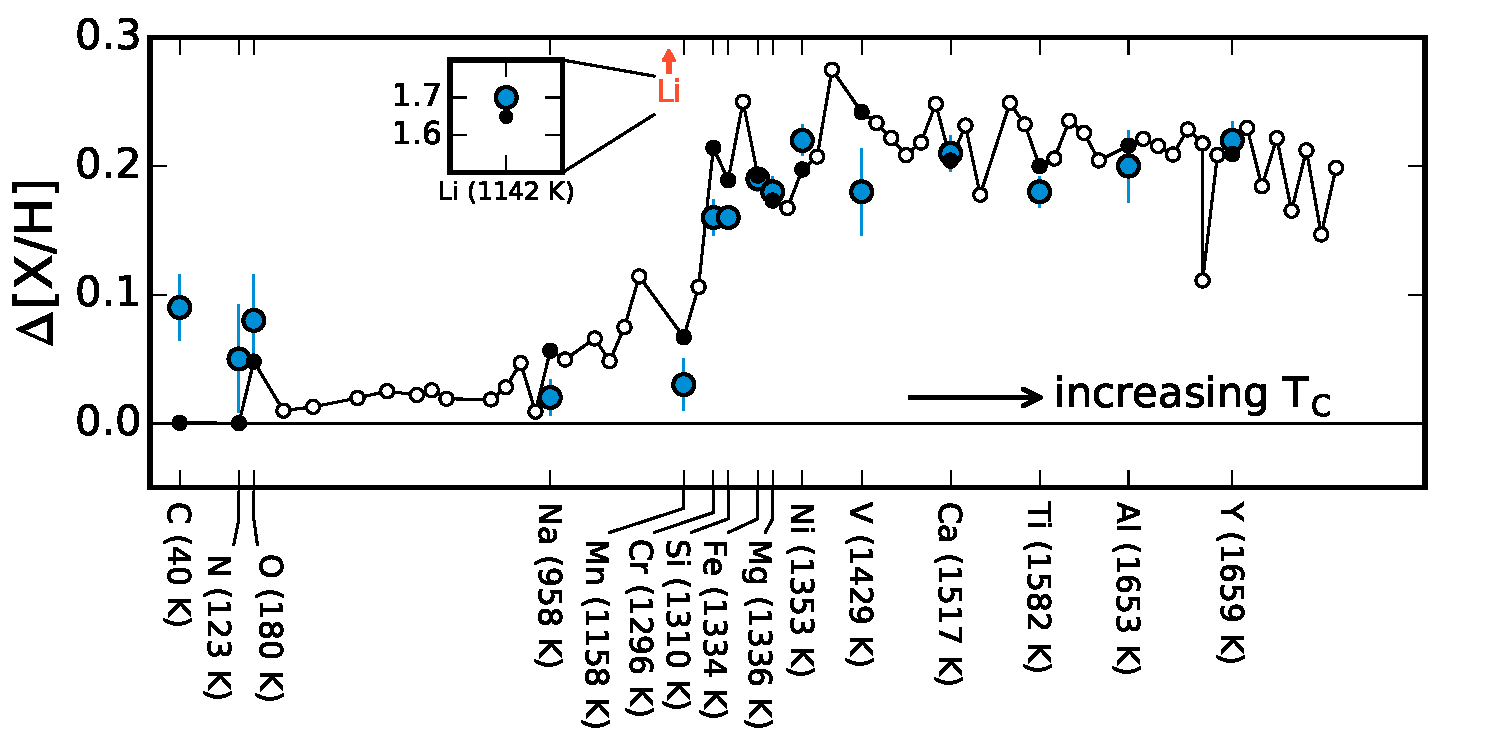
\includegraphics[width=0.95\linewidth]{deltaxh_tcrank.pdf}
  \caption{
    Comparing the observed abundance difference (blue circles) to the expected
    change in solar surface abundance after adding $15$~\mearth\ of material
    with bulk Earth composition\cite{2003TrGeo...2..547M} (black open and
    filled circles).
    The assumed mass fraction in the convective zone is $0.02$.
    All astronomical metals are ordered by their \Tcondens\ for solar
    composition gas on the $x$-axis.
    For the predictions, we highlight elements measured for \bizarreone-\sunanalog\ pair
    in filled circles, while those without a measurement are left open.
    The close match with the observed abundance difference in \bizarreone-\sunanalog\ pair
    suggests that the abundance difference may be due to accretion of
    $15$~\mearth\ of rocky planetary material.
    The element \elem{Li} is off the plot and indicated in the inset.
  }
  \label{fig:deltaxh_tcrank}
\end{figure}

Sorting the abundance differences by $50$\% condensation temperature ($T_C$) of the
elements shows a clear increasing trend.
In \figname~\ref{fig:deltaxh_tcrank},
we show the abundance difference between \bizarreone\ and \sunanalog\ ordered
by each element's equilibrium \Tcondens\ in solar system composition
gas\cite{2003ApJ...591.1220L}.
The five under-enhanced elements in \bizarreone\
relative to \sunanalog\ are the five most volatile of all elements measured.
The differences in \elem{Mn} ($\Tcondens = 1158$~K) and
\elem{Cr} ($\Tcondens = 1296$~K) suggest a break in $\Tcondens \approx 1200$~K.

We interpret the \Tcondens-dependent metal enhancement of \bizarreone\ relative
to \sunanalog\ and the very high surface \elem{Li} abundance ($A(\elem{Li}) =
2.75$) of \bizarreone\ as evidence for accretion of rocky (refractory-rich)
planetary material in \bizarreone.
In a multi-planet system, dynamical instabilities triggered by planet-planet
scattering\cite{1996Sci...274..954R,1996Natur.384..619W} or encounters with a
field star\cite{Malmberg:2011aa} can lead to planet ejection or accretion.
If one of the two stars in a wide binary accreted more refractory-rich (rocky) planets
than the other, this may imprint a strong \Tcondens-dependent
abundance differences like those observed in \bizarreone-\sunanalog.


%%TODO: cautions on condensation temperature
%% 1. it is just a proxy
%% 2. it is **equlibrium** condensation temperature


We estimate that the accretion of $\approx 15$~\mearth\ of rocky planets
in \bizarreone\ relative to \sunanalog\ can explain the enhancement in
refractory elements as well as the surface Li abundance.
Because the anchor star, \sunanalog,
is very similar to the Sun in its stellar properties (\teff, \logg, \feh, age),
we can use assume the Sun's photosphere abundances\cite{Asplund:2009aa} as the
pre-accretion state of \bizarreone.
In \figname~\ref{fig:deltaxh_tcrank}, we show the expected change in solar abundances,
$\Delta\elemH{X}$, after adding $15$~\mearth\ of bulk Earth composition
material\cite{2003TrGeo...2..547M} assuming that 2\% of the star's mass is in
its convective zone\cite{Pinsonneault:2001aa}.
It has long been known that more volatile (low \Tcondens) elements are more
depleted in the Earth relative to CI or other carbonaceous
chondrites\cite{mcdonough2001composition} that are thought to reflect the
elemental composition of the proto-solar nebula.
This trend is presumed to be closely related to the formation of terrestrial
planets and, in particular to the radial temperature gradient in a
protoplanetary disk.
The trend resulting from adding $15$~\mearth\ of bulk Earth provides an overall
good match to the observed $\Delta\elemH{X}$, suggesting that the
refractory-enhanced star, \bizarreone\, accreted $\approx 15$~\mearth\ more of
rocky planetary material than \sunanalog.

The accretion scenario can naturally explain the anomalously high
surface \elem{Li} abundance in \bizarreone.
Because \elem{Li} is strongly depleted in old sun-like stars, yet
present in bulk Earth with a concentration of $1.1$~ppm\cite{2003TrGeo...2..547M},
late-time accretion of rocky planetary material will significantly
replenish the lithium in the star's surface.
For the present-day Sun, the accretion of $15~\mearth$ of bulk Earth-like
material would result in $\Delta\elemH{Li} \approx 1.6$~dex
(see inset of \figname~\ref{fig:deltaxh_tcrank}).
Incidentally, the \bizarreone-\sunanalog\ system has an age (informed by
stellar parameters) very close to the Sun ($\sim 4$~Gyr).
Thus, as long as we believe the Sun's present-day surface \elem{Li} abundance
to be ordinary, the accretion of $15$~\mearth\ by \bizarreone\ is consistent with a $1.65$~dex
enhancement in \elem{Li} abundance.
This is exactly what we find: the \elem{Li} abundance of \bizarreone\ is
$A(\elem{Li}) = 2.75$ (Table~\ref{tab:t1}, Myles \etal, in prep.)
approximately $1.7$~dex higher than the solar value of $1.05$~dex\cite{Asplund:2009aa}.
While the current analysis of \elem{Li} line assumed a solar ratio of
$^{6}\elem{Li}/^{7}\elem{Li}$ given the data, we predict that a higher resolution
spectrum of the star will reveal a significant $^{6}\elem{Li}$ which are
normally destroyed early in solar-type stars, but present in rocky
planets\cite{Israelian:2001}.

\sunanalog\ is also enhanced in \elem{Li} compared to other stars of similar
ages by $\approx 1$~dex, considering its age of $4.00_{-1.56}^{+1.51}$~Gyr.
This enhancement puts an upper limit on the accreted mass to be
$\approx 4$~\mearth\ assuming a \elem{Li} concentration of $1.1$~ppm
\cite{mcdonough2001composition}, as above.
Unlike \bizarreone, we cannot know the pre-accretion abundances of
\sunanalog.\footnote{
  Strictly speaking, we can never know the pre-accretion abundances
  for \bizarreone\ either.
  We only have an {\it approximate} idea that this is not far from a solar-twin
  star \sunanalog, and because the deviation from this ``anchor'' star is
  large, it is reasonable to consider accretion by the Sun.
  In reality, \sunanalog\ may also have had its own accretion history,
  which indeed seems to be the case according to its \elem{Li} abundance.
}
However, we note that the span of abundance difference between highly volatile
elements (\elem{C}, \elem{N}, \elem{O}, \elem{Na}) and refractory elements such
as \elem{Fe} expected from accreting $4$~\mearth\ to the Sun is $\approx
0.05$~dex.
This is comparable to the abundance difference between N, Na, and Fe in
\sunanalog.
It is also interesting that \sunanalog\ shows a deficit in the same volatile
and moderately volatile elements (\elem{C}, \elem{N}, \elem{O}, \elem{Na}, and
\elem{Mn}) relative to Fe as in \bizarreone.
Thus, we conclude that \sunanalog\ is also likely to have had a similar
accretion event, but the amount of accretion was at least 5 times
smaller than \bizarreone.

What triggered the planet engulfment in the two comoving stars remains unclear.
One possibility is that a fly-by interaction with a field star could have
triggered eccentricity excitation of outer planets around each star, which may
have propagated inward through planet-planet scattering,
leading to the accretion of inner rocky planets\cite{Zakamska:2004aa,Malmberg:2011aa}.
If this is the case, there may be surviving, highly-eccentric giant planets.
The two stars have not been included in any publicly released data from planet
search programs, however, outer eccentric planets are potentially detectable
with future data releases of the \gaia\ mission.
If both stars have accreted planetary material, it would be very interesting to
search for the existence and architectures of the planetary systems left
behind.


\bibliography{ref}

\section{Acknowledgements}
We thank Andy Casey for bringing $^{6}\elem{Li}$ into our attention.
We thank Megan Bedell and Andy Casey for valuable discussions,
and Keith Hawkins, Nathan Leigh, and Josh Winn for comments
on early version of the draft.
The Flatiron Institute is supported by the Simons Foundation.
% Gaia
This work has made use of data from the European Space Agency (ESA) mission
{\it Gaia} (\url{http://www.cosmos.esa.int/gaia}), processed by the {\it Gaia}
Data Processing and Analysis Consortium (DPAC,
\url{http://www.cosmos.esa.int/web/gaia/dpac/consortium}). Funding for the DPAC
has been provided by national institutions, in particular the institutions
participating in the {\it Gaia} Multilateral Agreement.
% 2MASS
This publication makes use of data products from the Two Micron All Sky Survey,
which is a joint project of the University of Massachusetts and the Infrared
Processing and Analysis Center/California Institute of Technology, funded by
the National Aeronautics and Space Administration and the National Science
Foundation.
% all-WISE
This publication makes use of data products from the Wide-field Infrared Survey
Explorer, which is a joint project of the University of California, Los
Angeles, and the Jet Propulsion Laboratory/California Institute of Technology,
funded by the National Aeronautics and Space Administration.
% software
%\software{
%  %The data and code used in this project is available from
%  %\url{https://github.com/smoh/KronosKrios} under the MIT open-source
%  %software license.
%  This research utilized:
%  \texttt{Astropy} (\citealt{Astropy-Collaboration:2013}),
%  \texttt{emcee} (\citealt{2013PASP..125..306F}),
%  \texttt{IPython} (\citealt{Perez:2007}),
%  \texttt{matplotlib} (\citealt{Hunter:2007}),
%  \texttt{numpy} (\citealt{Van-der-Walt:2011}),
%  and \texttt{pandas} (\citealt{pandas}).}


\section{Extended Data}

\begin{figure}[htpb]
  \centering
  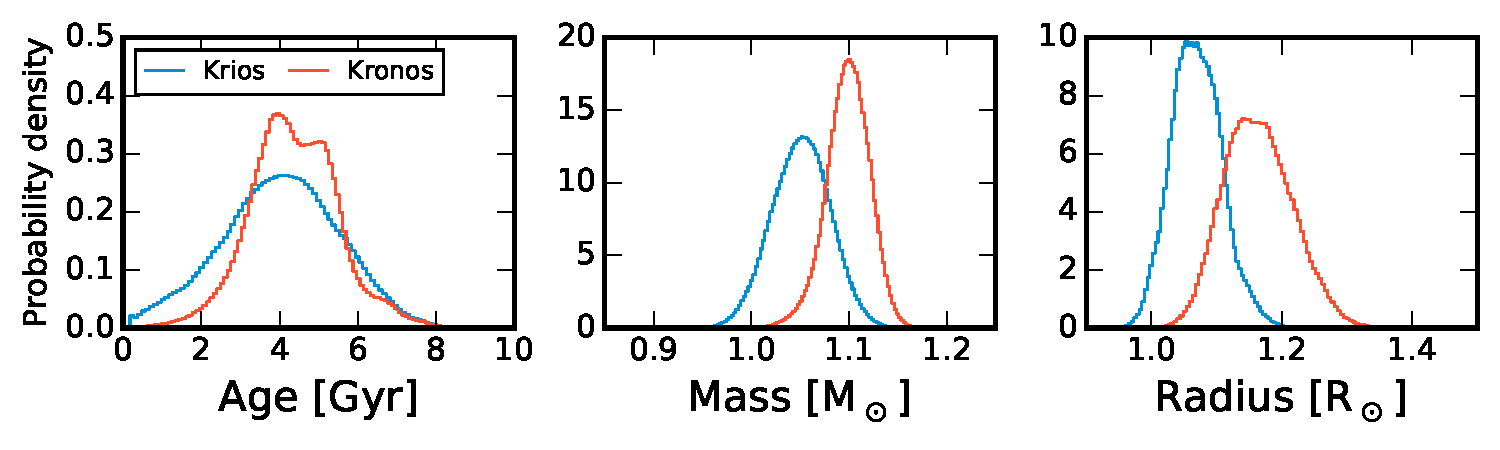
\includegraphics[width=0.95\linewidth]{yyisofitting.pdf}
  \caption{Probability density function of stellar age, mass, and radius
    from isochrone fitting using Yonsei-Yale isochrones\cite{2013ApJ...776...87S}
    and the star's luminosity, \teff, \feh, and \elemH{Si}.
  }
  \label{fig:yyisofitting}
\end{figure}


\begin{figure}[htpb]
  \centering
  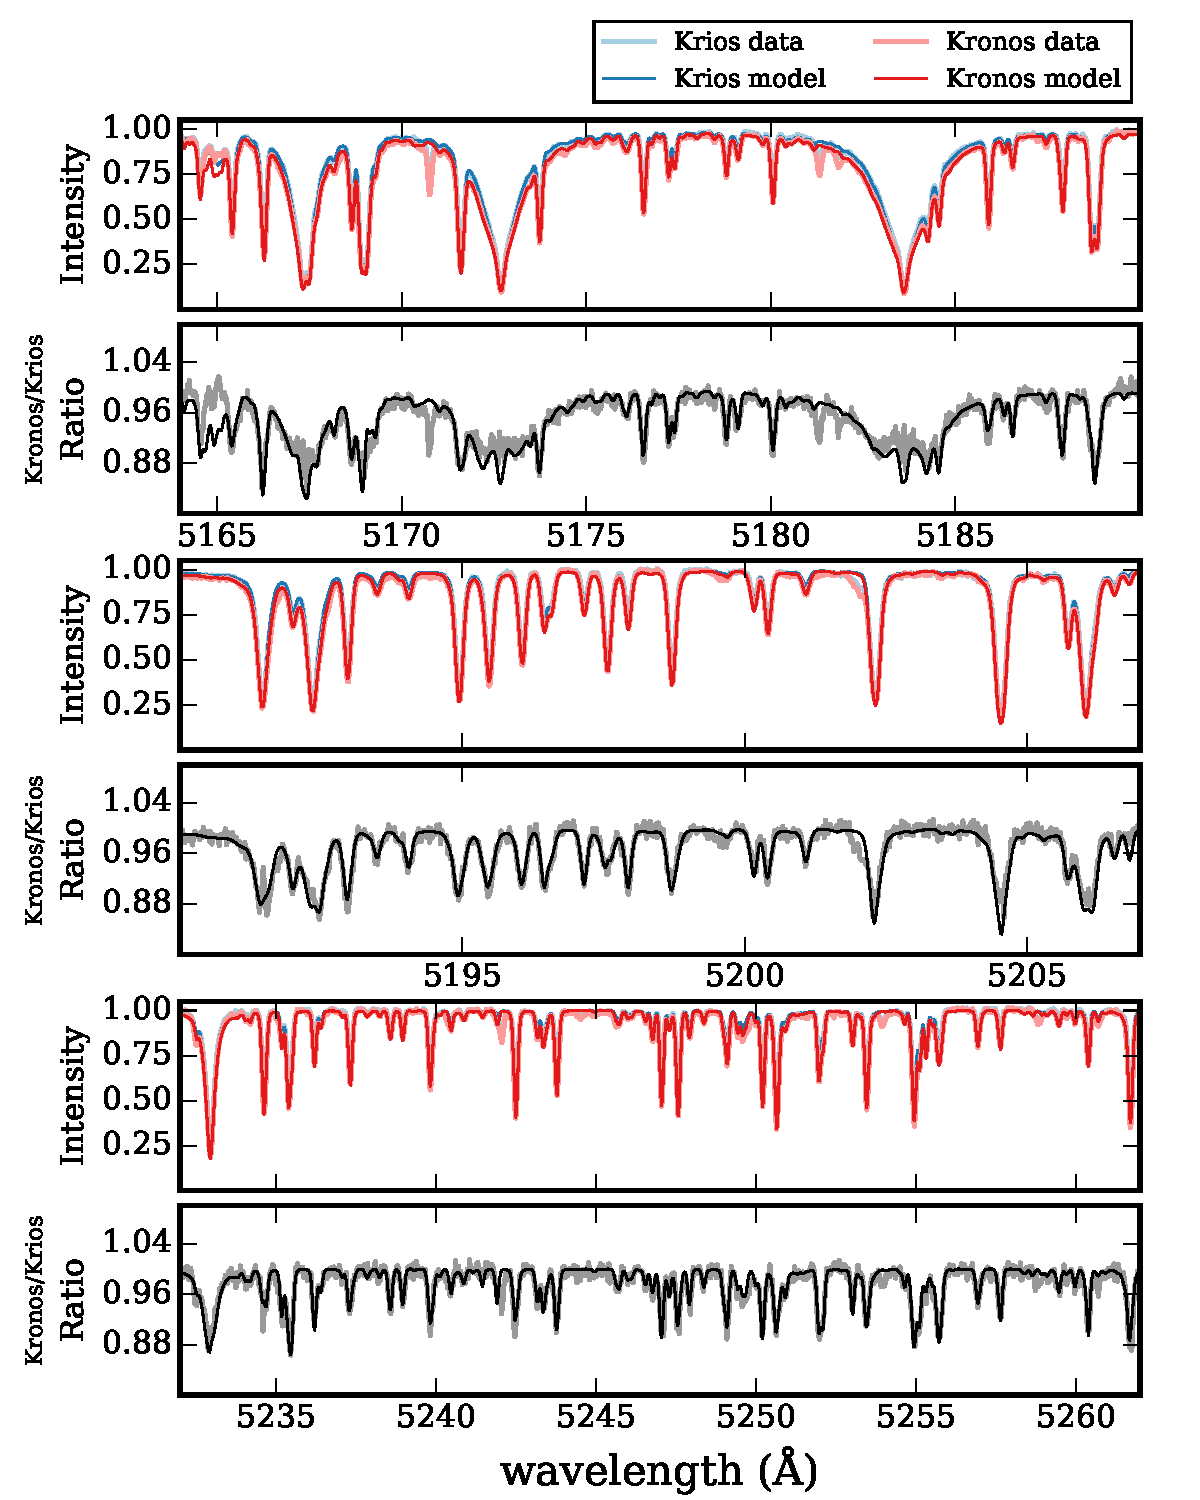
\includegraphics[width=0.95\linewidth]{spec1.pdf}
  \caption{Selective segments of the spectra of \sunanalog\ and \bizarreone.
    Alternating sets of two rows show
    the continuum-normalized data and model in the upper panel,
    and the ratio (\bizarreone/\sunanalog) of data (gray) and model (black)
    in the lower panel.
  }
  \label{fig:spec1}
\end{figure}

\begin{figure}[htpb]
  \centering
  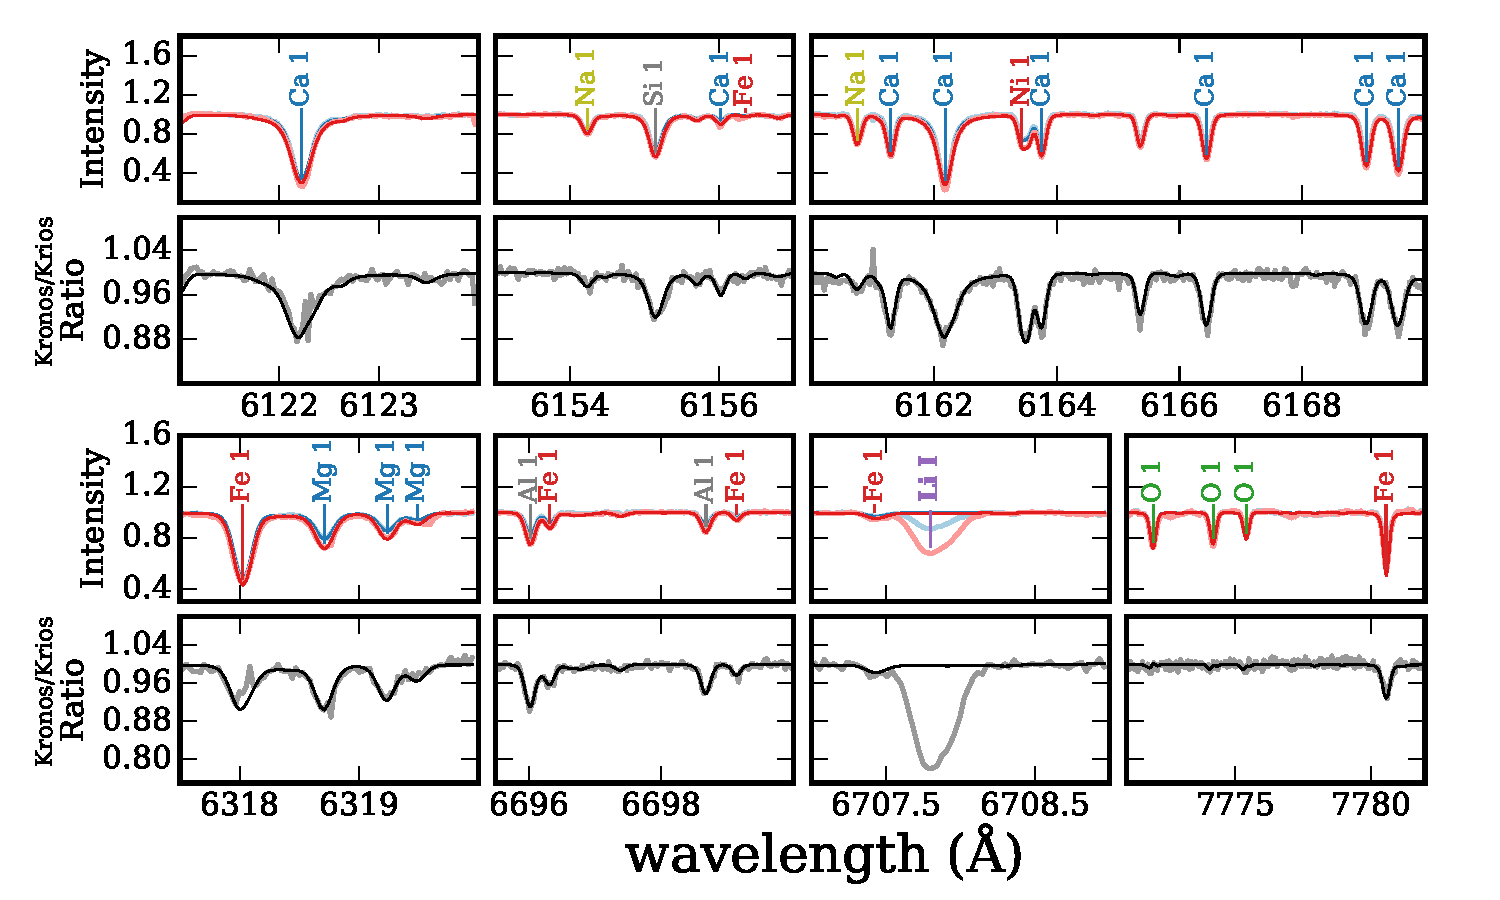
\includegraphics[width=0.95\linewidth]{spec2.pdf}
  \caption{Same as \figname~\ref{fig:spec1}
    but for smaller portions of spectra at longer wavelengths that are
    not dominated by \elem{Fe}.
    We mark elements that give rise to strong absorption lines.
    Note that the lines of \elem{Na} and \elem{O}, which are under-enhanced
    in \bizarreone\ relative to \elem{Fe} or other refractory elements,
    show noticeably weaker residuals compared to neighboring lines of
    refractory elements.
  }
  \label{fig:spec2}
\end{figure}

\begin{figure}[htpb]
  \centering
  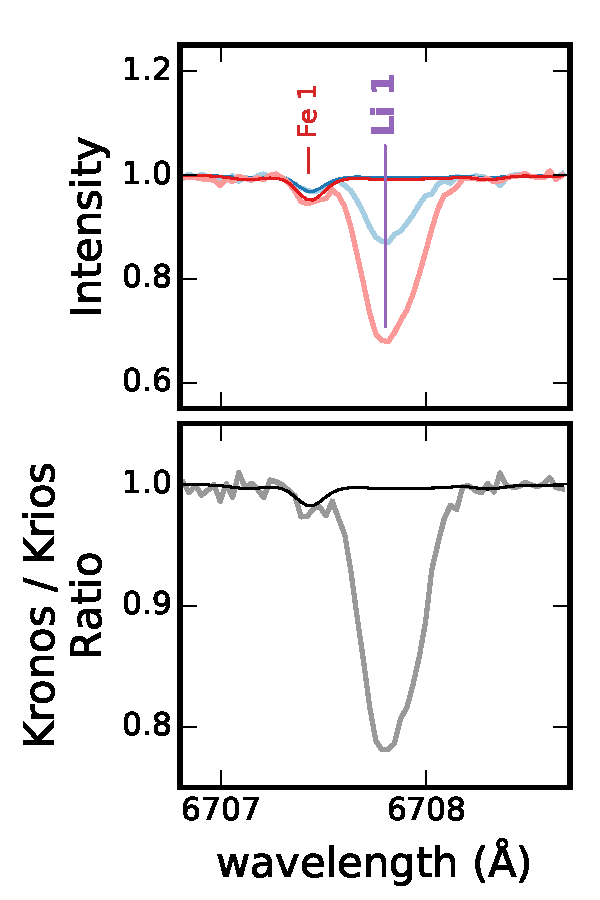
\includegraphics[width=0.6\linewidth]{spec_lithium.pdf}
  \caption{Lithium lines in the spectra of \bizarreone\ and \sunanalog.
    This line is studied in Myles \etal\ (in prep.).
    Line legends are the same as in \figname~\ref{fig:spec1}.
  }
  \label{fig:spec_lithium}
\end{figure}

\begin{figure}[htpb]
  \centering
  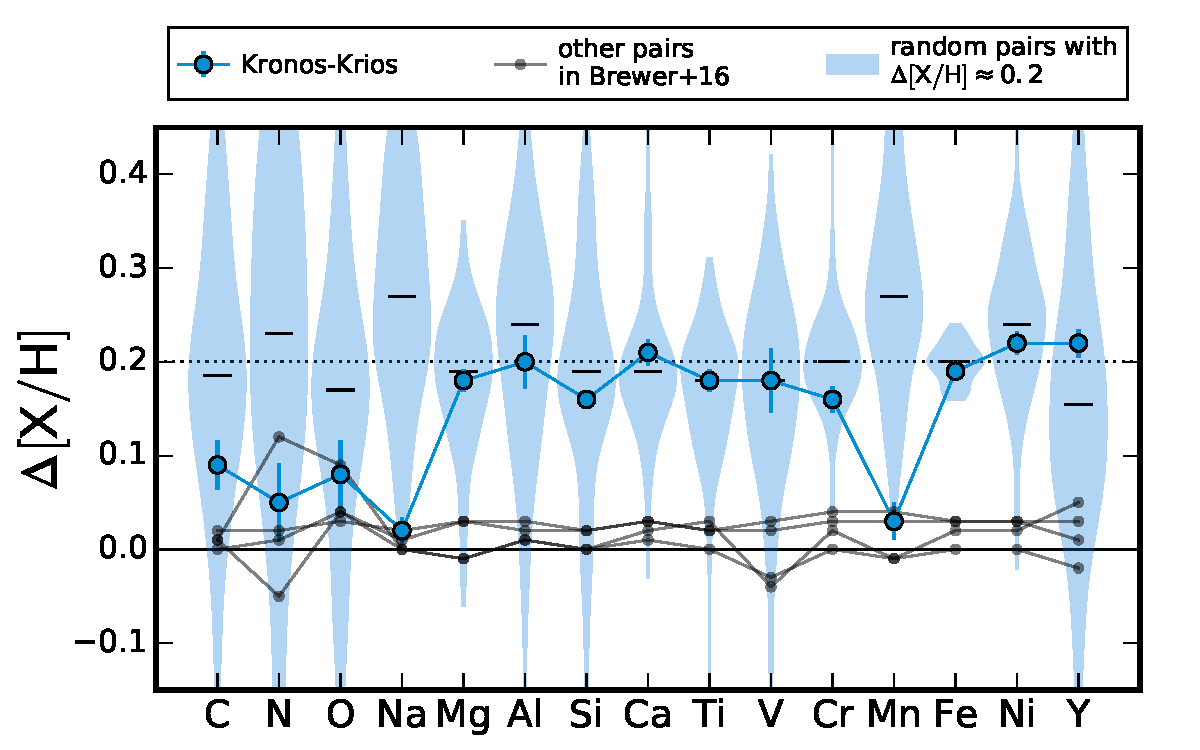
\includegraphics[width=0.95\linewidth]{deltaXH_elem_violins.pdf}
  \caption{Abundance difference in this pair (blue circles) and other twin-like
    ($\Delta T_\mathrm{eff}\lesssim 100$~K) wide binaries\cite{2016ApJS..225...32B}
    (black circles).
    The differences in other pairs are small ($<0.05$~dex)
    for all elements except \elem{N} and \elem{O} which are the most
    uncertain, making the difference of $\approx 0.2$~dex seen in
    \bizarreone-\sunanalog\ rare.
    Additionally, we show the distribution of abundance differences
    between field stars in the same catalog\cite{2016ApJS..225...32B}
    with similar metallicity difference
    ($\Delta[\elem{Fe}/\elem{H}] \approx 0.2$)
    as violins (shaded regions) with medians indicated by black line segments.
    These are random pairings of single stars from two metallicity bins,
    $-0.025 < \feh < 0.025$ (160 stars) and $0.175 > \feh > 0.225$ (137 stars),
    similar to \bizarreone\ and \sunanalog.
    The difference is always taken to be
    $\mathrm{higher}\,\feh - \mathrm{lower}\,\feh$.
    Thus, the narrower range of in $\Delta\feh$ is by construction.
    Random pairings of disk stars with similar $\Delta\feh$ usually show
    similar enhancement in all other elements
    unlike the pattern seen in \bizarreone-\sunanalog\ pair.
  }
  \label{fig:deltaXH}
\end{figure}


%As shown in \figname~\ref{fig:deltaXH},
%the differences in other pairs for all elements except \elem{N} and \elem{O},
%which are also the most uncertain (\tablename~\ref{tab:kk}),
%are less than $0.05$~dex, making \bizarreone-\sunanalog\ pair a significant outlier.

\begin{figure}[htpb]
  \centering
  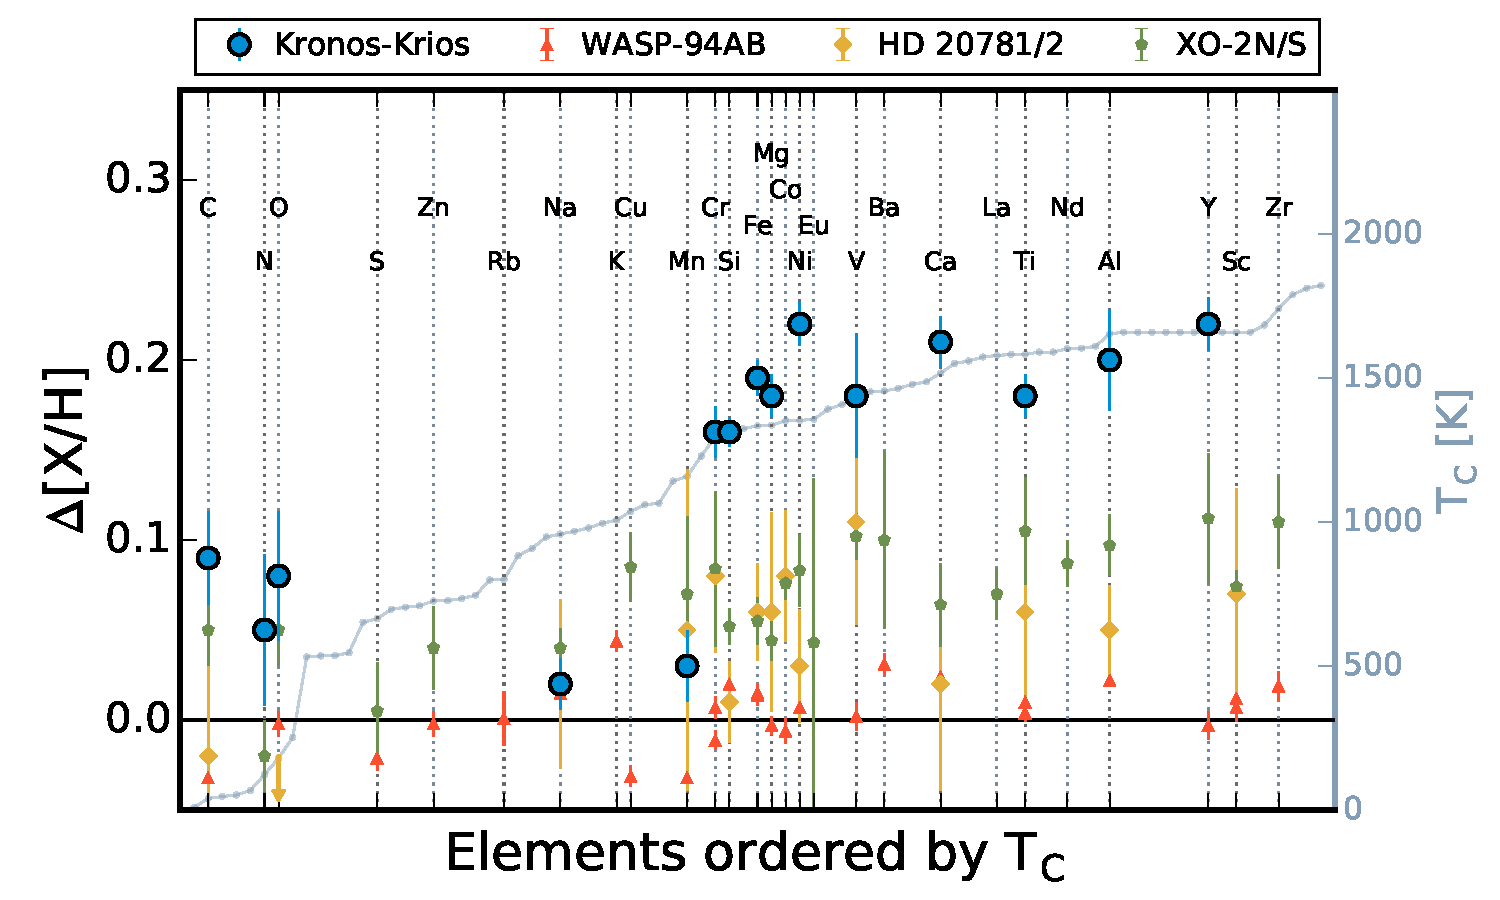
\includegraphics[width=0.95\linewidth]{TcRank_deltaXH_concise.pdf}
  \caption{Comparison to other pairs that show abundance differences.
    %TODO
    Abundance differences of the \bizarreone-\sunanalog\ pair ranked by the
    condensation temperature of elements for solar composition
    gas\cite{2003ApJ...591.1220L}.
    The condensation temperature may be read from the gray line and right y-axis.
    We show three wide binary systems selected from the literature:
    HD~20782/1\cite{Mack:2014aa} ($\feh\approx0$),
    XO-2N/S\cite{Biazzo:2015aa} ($\feh\approx0.35$),
    and WASP-94AB\cite{Teske:2016aa} ($\feh\approx0.3$).
    Locations of elements with at least one measurement from any study
    are indicated by a vertical line and its symbol.
    Note that often multiple values are reported for one element corresponding
    to different ionization states in equivalent width analyses.
    No other pair studied so far were shown to have such large difference
    in metallicity or sharp contrast between (moderately) volatile and
    refractory elements as \bizarreone-\sunanalog.
  }
  \label{fig:relabun_tcrank}
\end{figure}


\clearpage

\section{Supplementary Information}

\subsection{Proximity in phase-space coordinates}
\label{supp:dxdv}

\begin{figure}[htbp]
  \begin{center}
    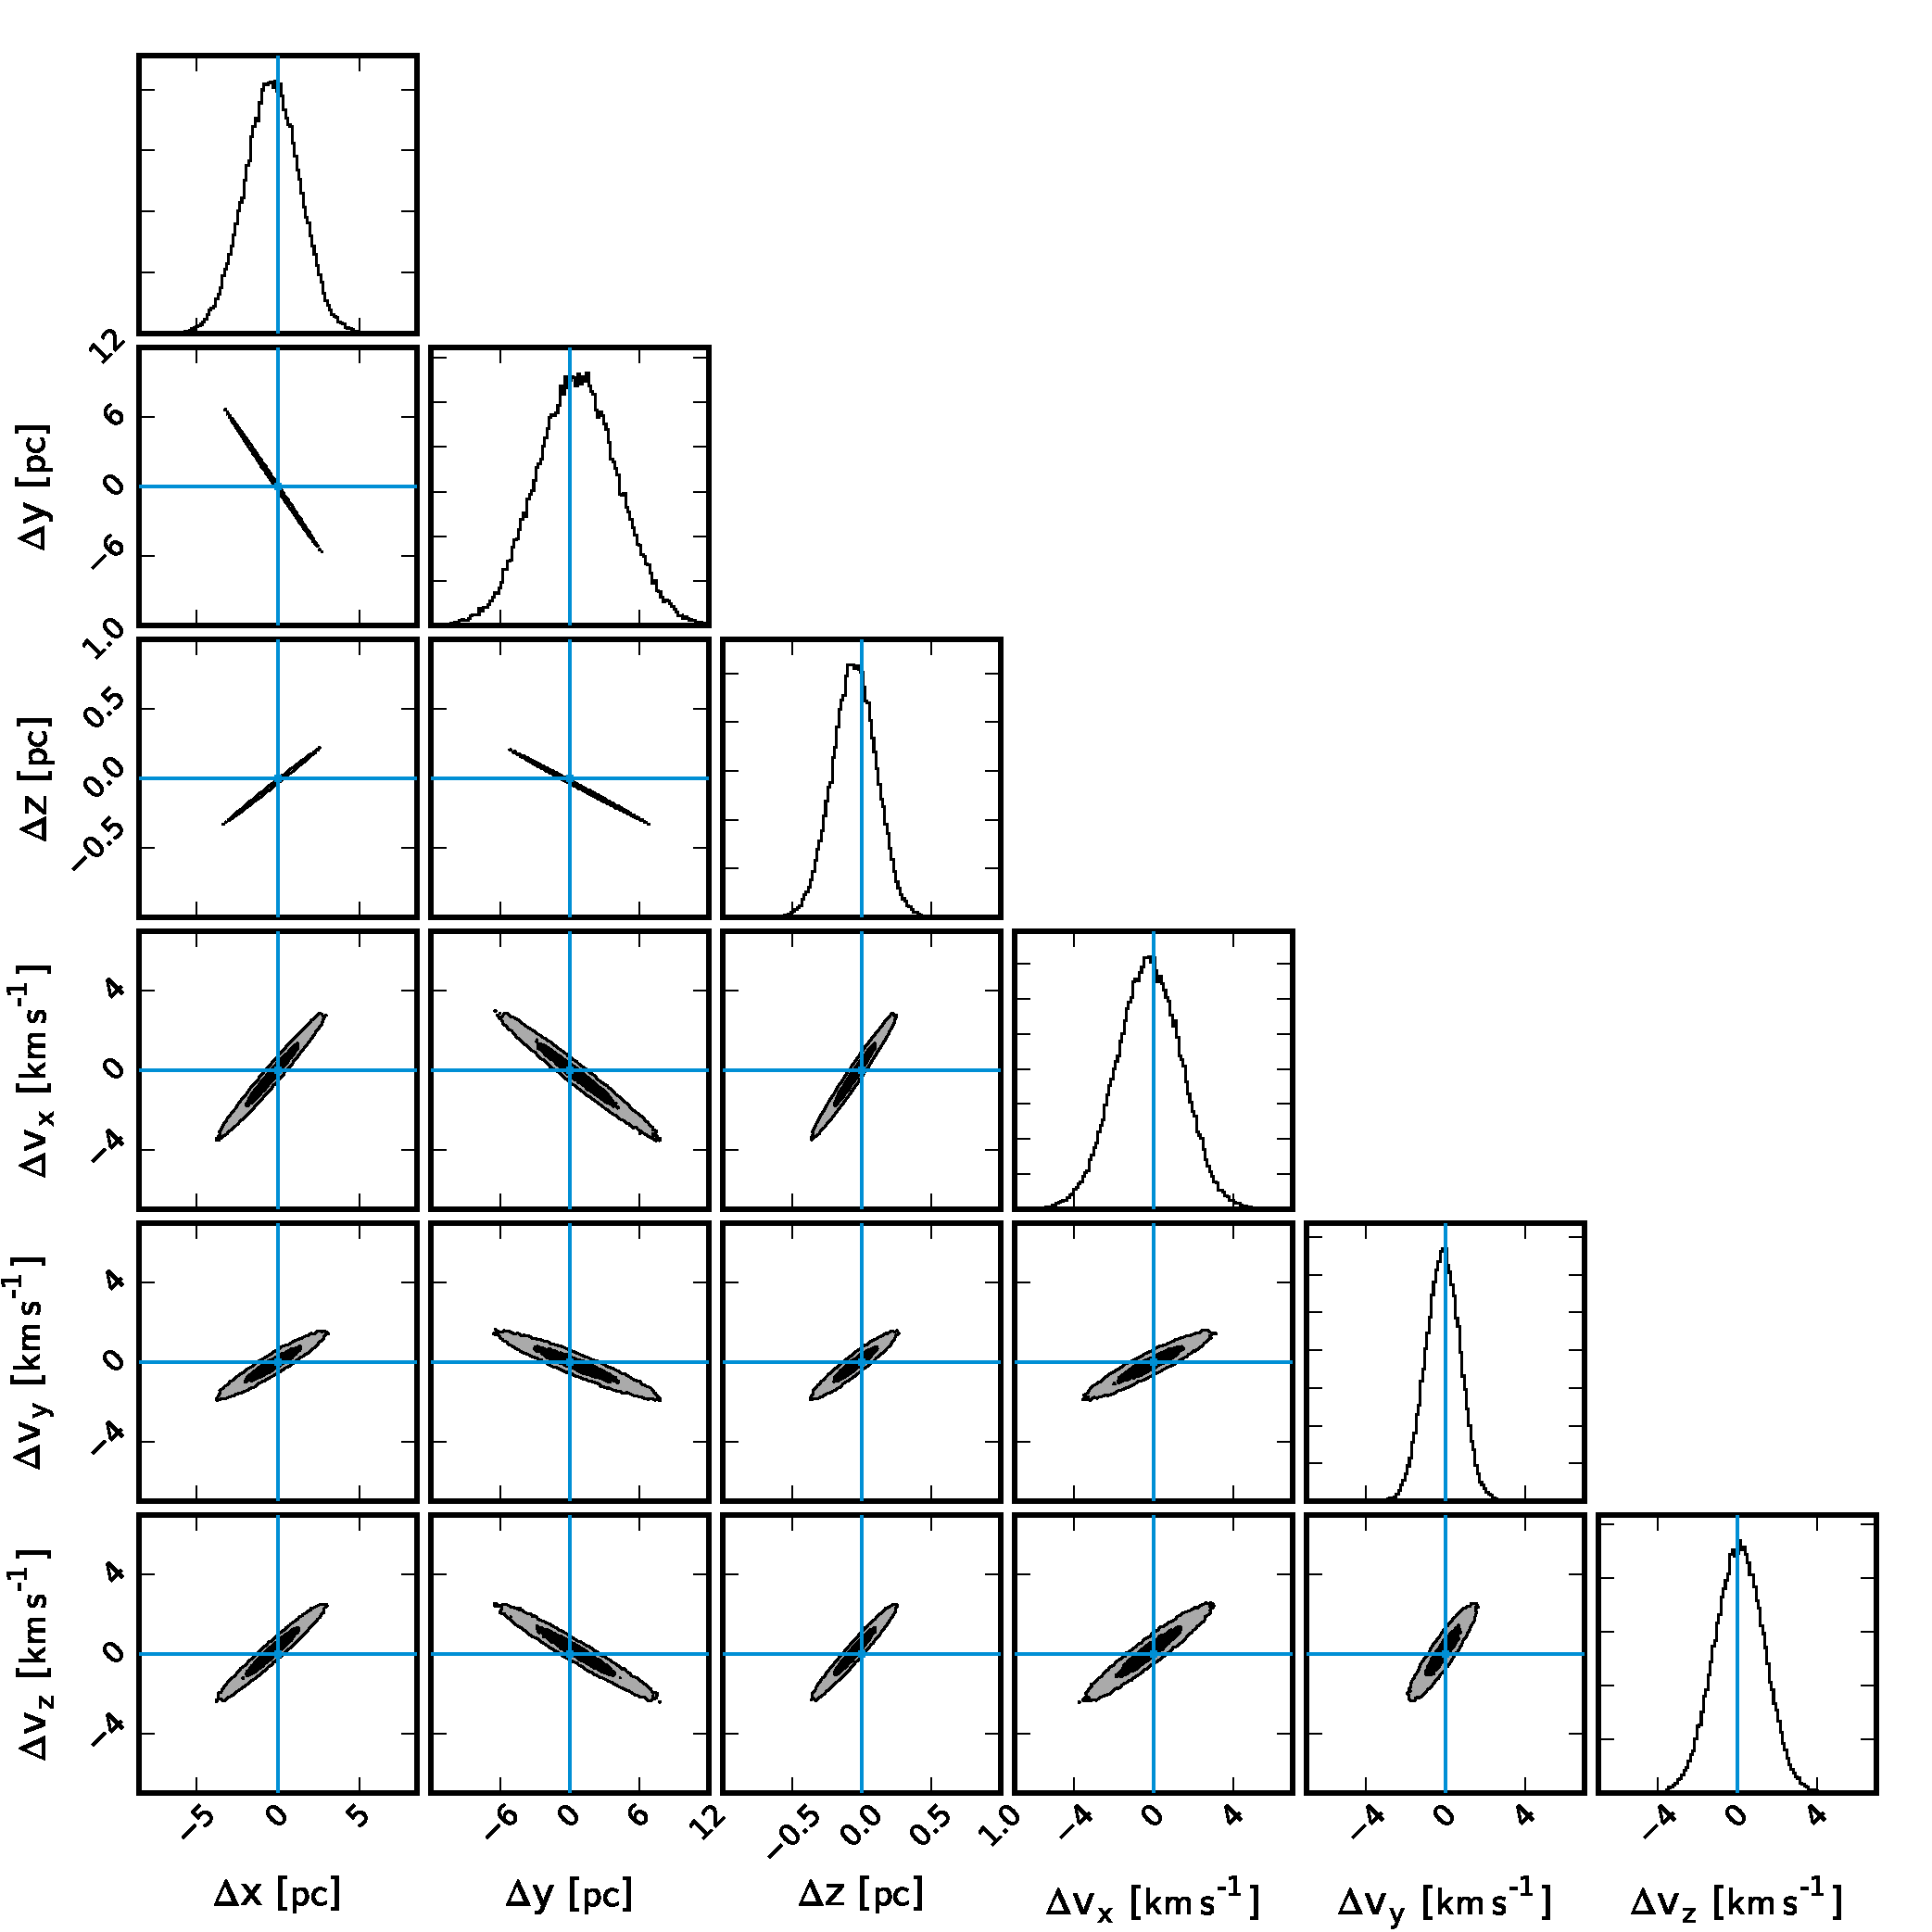
\includegraphics[width=\linewidth]{dx_dv_posterior.pdf}
  \end{center}
  \caption{%
    Differences in posterior samples over Galactocentric phase-space coordinates
    for the two stars, \bizarreone\ and \sunanalog.
    \label{fig:dxdv}}
\end{figure}

Combining the precise radial velocities obtained from spectra with the \tgas\
astrometry, we can compare differences between the inferred 6D phase-space
coordinates of the two stars.
We start by generating posterior samples over the Heliocentric distance, $r$,
tangential velocities, $(v_\alpha, v_\delta)$, and radial velocity, $v_r$,
given the observed parallax, $\hat\pi$, and proper motions,
$(\hat\mu_{\alpha^*}, \hat\mu_\delta)$, and radial velocity, $\hat v_r$.
We assume the noise is Gaussian, and the radial velocity measurement is
uncorrelated with the astrometric measurements.
If we define
\begin{eqnarray}
  \vec{\hat y} &=&
      \transp{\left(
        \begin{array}{c@{\hspace{1em}} c@{\hspace{1em}} c@{\hspace{1em}} c}
          \hat\pi &
          \hat\mu_{\alpha^*} &
          \hat\mu_\delta &
          \hat v_r
        \end{array}
      \right)}\\
  \vec{y} &=&
      \transp{\left(
        \begin{array}{c@{\hspace{1em}} c@{\hspace{1em}} c@{\hspace{1em}} c}
          r^{-1} &
          r^{-1}\,v_\alpha &
          r^{-1}\,v_\delta &
          v_r
        \end{array}
      \right)}
\end{eqnarray}
then the likelihood is
\begin{equation}
  \vec{\hat y} \sim \mathcal{N}(\vec{y}, \mat{C})
\end{equation} where $\mat{C}$ is the covariance matrix, and $\mathcal{N}$ is
normal (Gaussian) distribution\cite{2017AJ....153..257O}.
We adopt a uniform space-density prior for the distance and an isotropic
Gaussian for any velocity component, $v$, with a dispersion $\sigma_v=25~\kms$:
\begin{eqnarray}
p(r) &=&
  \begin{cases}
    \frac{3}{r_{\rm lim}^3} \, r^2 & \text{if } 0 < r < r_{\rm lim}\\
    0              & \text{otherwise}
  \end{cases}\\
p(v) &=& \frac{1}{\sqrt{2\pi}\,\sigma_v} \,
  \exp\left[-\frac{1}{2} \, \frac{v^2}{\sigma_v^2} \right] \quad .
\end{eqnarray}
%
For each of the two stars, we use \project{emcee}\cite{2013PASP..125..306F}
to generate posterior samples in $(r, v_\alpha, v_\delta, v_r)$
by running 64 walkers for 4608 steps and discarding the first
512 steps as the burn-in period.
For each sample, we convert the Heliocentric phase-space coordinates into
Galactocentric coordinates assuming that the Sun's position and velocity are
$\vec x_\odot = (-8.3,\,0,\,0)~{\rm kpc}$ and $\vec v_\odot =
(-11.1,\,244,\,7.25)~\kms$\cite{Schonrich:2010, Schonrich:2012}.

\figurename~\ref{fig:dxdv} shows differences in posterior samples converted to
Galactocentric phase-space coordinates for the two stars.
The differences in positions and velocities are consistent with zero.
% \todo{should we instead show $|\Delta\boldsymbol{x}|$ and
% $|\Delta\boldsymbol{v}|$ computed from the 6D posterior samples?}

\subsection{Stellar Ages and Coevality}
\label{sub:age_coevality}

\begin{figure}[htbp]
  \begin{center}
    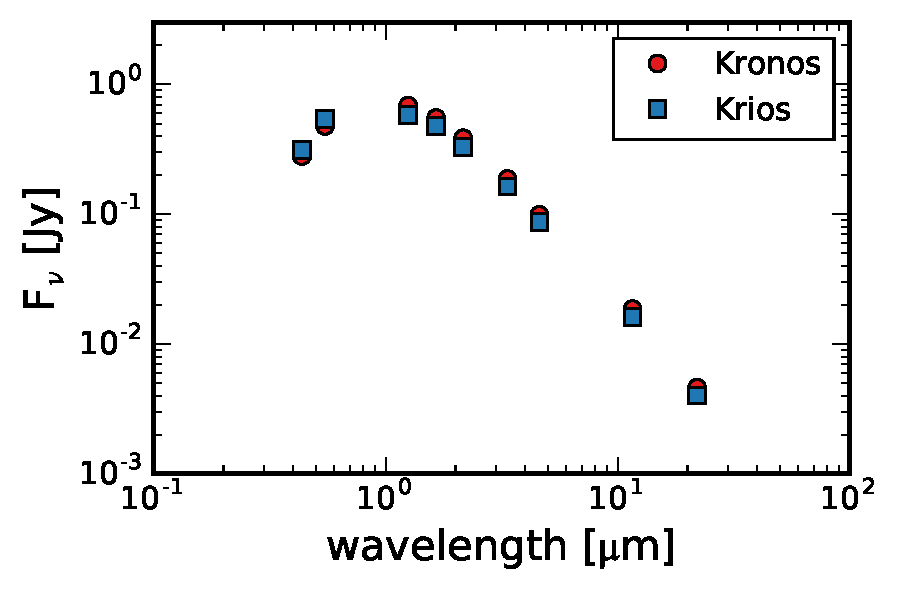
\includegraphics[width=0.65\linewidth]{sed.pdf}
  \end{center}
  \caption{Spectral energy distributions of \bizarreone\ and \sunanalog.
    We compiled the photometric measurements from
    \project{Tycho-2}\cite{2000A&A...355L..27H},
    \project{2MASS}\cite{2006AJ....131.1163S}, and
    \project{WISE}\cite{2010AJ....140.1868W}.
  }
  \label{fig:sed}
\end{figure}

\begin{figure}[htbp]
  \begin{center}
    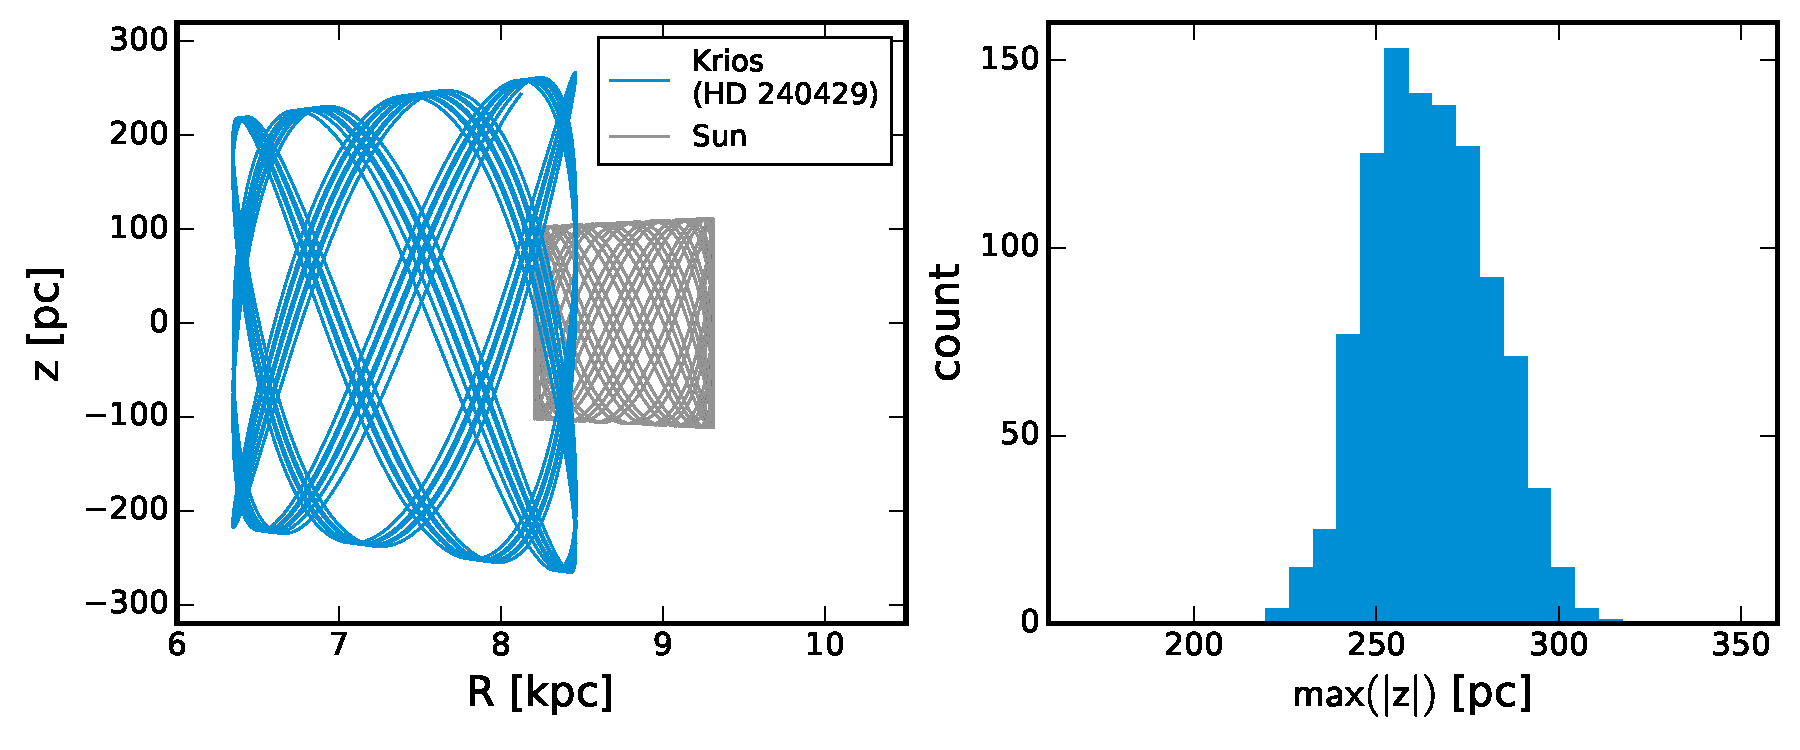
\includegraphics[width=\linewidth]{orbits.pdf}
  \end{center}
  \caption{Left panel: Galactic orbits computed for \sunanalog\ (blue) and the
    Sun (grey).
    For \sunanalog, the initial condition is set to the median of the
    posterior samples over the phase-space coordinates.
    The orbits are computed by integrating backwards from the present-day
    positions for $2.5$~Gyr with a time step of $0.5$~Myr using the Leapfrog
    integration scheme implemented in \project{Gala}\cite{gala}.
    Right panel: Distribution of maximum $z$-heights for orbits computed from
    all posterior samples for \sunanalog.
    The large $z$-height is consistent with an old ($\sim 4$~Gyr) age
    (\sectionname~\ref{sub:age_coevality}).
  }
  \label{fig:orbit}
\end{figure}

We provide a more detailed discussion of stellar ages and coevality of
\bizarreone-\sunanalog\ pair, aside from the isochrone fitting,
especially on whether the stars may be very young ($\lesssim 1$~Gyr).
The surface lithium abundance in a sun-like star decreases with its age due to
mixing induced by convection or rotation, which brings the lithium into the
interior ($T>2.5 \times 10^{6}$~K) where it will be destroyed by proton capture
burning.
Thus, surface lithium abundance can be an indicator of stellar ages.
The absolute $\elem{Li}$ abundance of $2.25$~dex for \sunanalog\ implies an age
of $\lesssim 1$~Gyr according to the theoretical models tuned to explain the
solar lithium abundance and rotational profile\cite{2005Sci...309.2189C}.
The lithium abundance of \bizarreone\, $2.74$~dex, shows the largest difference
among all measured elements.
This translates to a $\sim 500$~Myr difference in age.
Given the overall higher metal abundances and the peculiar abundance patterns
in \bizarreone, it is unclear, however, whether this higher $\elem{Li}$
abundance means a younger age or something else.
For example, the presence of $\elem{Li}$-rich red giant stars was
attributed to the engulfment of substellar companions such as gas giant planets
or brown dwarfs which may replenish $\elem{Li}$\cite{Casey:2016aa}.

The surface lithium abundance is the only indicator of a
younger age.
If the two stars were only several hundred Myrs old, then they would likely
have been part of a larger comoving group of stars.
However, there is no evidence in our search\cite{2017AJ....153..257O} of
comoving pairs using \tgas\ that these stars belong to a larger group of
young stars.
Very young stars often show signs of activity such as
X-ray emission from magnetic activity, emission lines, or infrared excess due to
circumstellar disks (\todo{needs refernces}).
We have compiled GALEX, Tycho-2, 2MASS, and WISE photometry for these stars, and
found no evidence for indications of activity or infrared excess in their
spectral energy distributions (\figname~\ref{fig:sed}).
The low $v\sin(i)$ values (\tablename~\ref{tab:t1}) also argue against very
young ages that would be inferred from the surface lithium abundances.
Finally, we computed the Galactic orbit of the pair using the median of the
posterior sample over the phase space coordinates of \sunanalog, in a Milky
Way-like gravitational potential\cite{Bovy:2015} using \project{Gala}\cite{gala}.
The pair's fiducial orbit has a vertical action larger than the Sun, favoring
an older age (\citealt{Wielen:1977,Aumer:2016}); see \figname~\ref{fig:orbit}.
We therefore conclude that the two stars are most likely coeval, $\sim 4$~Gyr
old main sequence stars, and that their unusually high \elem{Li} abundance
requires an alternative explanation; our favored explanation being the accretion
of rocky material that has locked lithium.

\subsection{Alternative Scenarios}

\subsubsection{Exchange Scattering}
\label{sub:exchange_scattering}

While the data described above strongly suggests that the two stars are
coeval, this subsection explores the possibility that this is not a primordial
binary.
Two stars unrelated at birth may end up in a binary system via a binary-single
scattering event that results in an exchange of binary members.
In order to estimate the rate at which any binary-single
event will produce a wide binary system such as \sunanalog\ and \bizarreone,
we may consider the rate at which this wide binary will scatter with a field star to
result in an exchange reaction.
The cross-section of exchange scattering for a binary with semi-major axis $a$ is
\cite{Hut:1983ab,Hut:1983aa}
\begin{eqnarray}
  \sigma_\mathrm{ex} = \frac{640}{81} \pi a^{2} \left(\frac{v_i}{v_c}\right)^{-6}
  \label{eq:crosssection}
\end{eqnarray}
where $v_i$ is the incoming velocity, and $v_c$ is the critical velocity,
defined as
\begin{eqnarray}
  v_c^2 = G \frac{m_1 m_2 (m_1 + m_2 + m_3)}{m_3 (m_1 + m_2)} \frac{1}{a}\,\,.
\end{eqnarray}
\eqname~\ref{eq:crosssection} is appropriate when $v_i/v_c \gg 1$,
which is the case for wide binaries
scattering with field (disk) stars.
If we assume that field stars are made of solar mass stars with a constant
number density $n=1$~pc$^{-3}$, and the incoming velocity of field stars is
$10$~\kms, the rate of exchange scattering is
\begin{eqnarray}
  n \sigma_\mathrm{ex} v_i = 6.82\times 10^{-8}\,\mathrm{Gyr}^{-1}
  \frac{n}{\mathrm{pc}^{-3}} \frac{\mathrm{pc}}{a}
  \left(\frac{10~\mathrm{km}\,\mathrm{s}^{-1}}{v_i}\right)^5\,,
\end{eqnarray}
which is low enough to be negligible.
This is a conservative estimate as the relative velocity of
disk stars exceeds $10$~\kms.

An exchange scattering scenario is unlikely to be able to explain the observed
abundance difference pattern.
We test this by comparing the observed abundance difference of
\bizarreone-\sunanalog\ with the distribution of abundance differences,
$\Delta[\elem{X}/\elem{H}]$, between pairs of two stars randomly drawn
from two metallicity (\feh) bins similar to \bizarreone\ and \sunanalog\
(\figname~\ref{fig:deltaXH}).
We see that when a star is enhanced in $\elem{Fe}$ by $0.2$~dex,
all other elements are typically enhanced at a similar level, with some variations.
Specifically, for a typical star with $\feh \approx 0.2$~dex, we generally
expect $[\elem{Na}/\elem{Fe}] > 0$ and $[\elem{Mn}/\elem{Fe}] > -0.1$
\cite{Battistini:2015aa,Bensby:2003aa}, making the low
[\elem{Na}/\elem{Fe}] and [\elem{Mn}/\elem{Fe}] seen in \bizarreone\ very
unlikely to arise from variations in Galactic chemical evolution.


\subsubsection{Chemical Inhomogeneity in Star Formation}
\label{sub:chemical_inhomogeneity_in_star_formation}

In this subsection, we explore the hypothesis that the chemical inhomogeneity
within the birth cloud is the source of the \bizarreone-\sunanalog\ abundance
anomalies.
There is ample evidence against this scenario.
None of the other seven similar wide binaries examined
with the same measurement pipeline\cite{2016ApJS..225...32B}
show the same level of differences in abundances.
Though there is generally a larger spread in $\elem{C}$, $\elem{N}$ and
$\elem{O}$, and some pairs show a difference in particular elements as large as
$\approx 0.15$~dex.
The median and maximum \feh\ difference between component stars in the other
seven pairs is $0.02$~dex and $0.09$~dex, respectively.
The differences are even smaller (maximum $\Delta\feh = 0.03$~dex) if we
compare only twin-like ($\Delta T_\mathrm{eff} \lesssim 100$~K) pairs
(\figname~\ref{fig:deltaXH}).
This is consistent with similar previous studies\cite{Gratton:2001aa,Desidera:2004aa}.
Thus, a difference of $\approx 0.2$~dex seen in \bizarreone-\sunanalog\ pair is
not likely due to chemical inhomogeneity in the birth cloud.


\subsection{Estimating the accreted masses}

\begin{figure}[htpb]
  \centering
  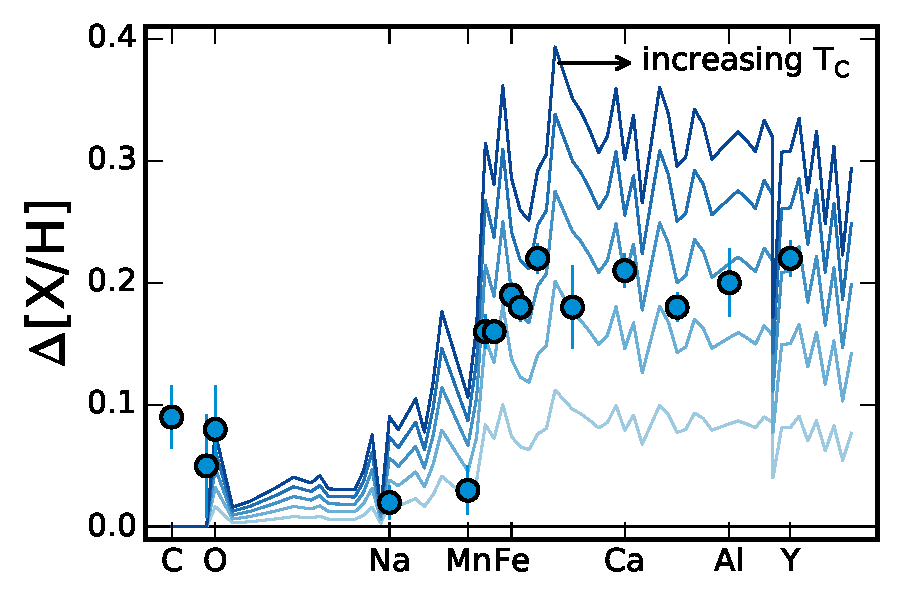
\includegraphics[width=0.95\linewidth]{deltaxh_tcrank_vari.pdf}
  \caption{Expected differences in solar abundances after adding
    varying mass of bulk Earth material.
    Elements are ordered by their $T_C$ on $x$-axis, same as
    \figname~\ref{fig:deltaxh_tcrank}.
    We assume $f_\mathrm{CZ} = 0.02$ and show expected $\Delta\elemH{X}$
    for adding 5, 10, 15, 20, 25~\mearth\ of bulk Earth (from bottom to top).
  }
  \label{fig:vari}
\end{figure}

We estimate how much added rocky material is needed to explain an
increment of $\approx 0.2$~dex in refractory elements observed in \bizarreone\
relative to \sunanalog\cite{Mack:2014aa,Mack:2016aa}.
Because \sunanalog\ is a solar-twin star in that its $T_\mathrm{eff}$, \logg,
and \feh\ is very close to those of the Sun ($\Delta T_\mathrm{eff} \approx XX$,
$\delta\logg \approx XX$, and $\Delta\feh \approx 0$),
we may approximate the pre-accretion abundances of \bizarreone\ as being
equivalent to the sun.
We carry out simple toy calculations of expected $\Delta\elemH{X}$
in a Sun-like star's atmosphere by adding a certain mass of bulk Earth
composition under these simplifying assumptions:
\begin{itemize}
  \item The material added is instantly and completely mixed.
  \item The atmospheric composition that we measure is identical throughout
    the star's radiative and convective zone.
  \item The surface abundance of the star has been altered only by the
    accretion event(s).
\end{itemize}
We take the solar abundances\cite{Asplund:2009aa}, $\elemH{X}$, of element \elem{X}
which can be converted to mass fraction as
\begin{equation}
  f_{X,\mathrm{photo}} = \frac{10^{\elemH{X}} m_X}{\Sigma_X 10^{\elemH{X}} m_X}
\end{equation}
where $m_X$ is the mass of each element in, e.g., atomic mass unit.
Assuming that the added material has a total mass $M_\mathrm{add}$, and the
mass fraction in each element is $f_{X,\mathrm{add}}$,
the abundance difference is
\begin{equation}
  \Delta\elemH{X} = \log_{10} \frac{f_{X,\mathrm{photo}}\,f_\mathrm{CZ}\,M_\mathrm{star}
    + f_{X,\mathrm{add}}\,M_\mathrm{add}}
    {f_{X,\mathrm{photo}}\,f_\mathrm{CZ}\,M_\mathrm{star}}
\end{equation}
where $f_\mathrm{CZ}$ is the fraction of the star's mass in the convective envelope.
We take the composition of bulk Earth\cite{mcdonough2001composition}
as a proxy for rocky planet composition. We adopt $f_\mathrm{CZ} = 0.02$ for
the fraction of mass in the convective zone\cite{Pinsonneault:2001aa}.

The estimate of accreted mass depends sensitively on $f_\mathrm{CZ}$ and the
mass of the star which are difficult quantities to constrain directly through
data.
We adopt $(f_\mathrm{CZ},\,M) = (0.02, 1~M_\odot)$, and show
expected changes for the accretion of $5-25$~\mearth\ of bulk Earth material
in \figname~\ref{fig:vari}.
However, we note that if $f_\mathrm{CZ}$ is $0.03$, the estimate for the accreted
mass would be $\approx 20$~\mearth.

We stress that while the calculation carried out is useful in
an order-of-magnitude sense, further investigation of each of the simplifying
assumptions made is warranted.
In addition, the composition of bulk Earth has some uncertainties.
For example, the reported bulk Earth concentration of \elem{Mn}, varies from
$800$ to $1700$~ppm\cite{1998psc..book.....L,mcdonough2001composition,2003TrGeo...2..547M}
largely due to uncertainties in the composition of the Earth's core.
Given these limitations, the level of agreement for $\Delta\elemH{X}$ {\it and}
\elem{Li} for \bizarreone\ is remarkable.

%\begin{deluxetable*}{c|cccc}
  \tablecaption{Astrometric and spectroscopic measurements of the pair
  \label{tab:kk}}
\tablehead{
  \colhead{}     & \colhead{}      & \sunanalog\         & \bizarreone\        & \colhead{} \\
  \colhead{Name} & \colhead{Units} & \colhead{HD 240429} & \colhead{HD 240430} & \colhead{Uncertainties}
}
\startdata
Sp Type                             &                & G0                     & G2                     &       \\
R.A.\tablenotemark{a}               & hh:mm:ss       & 23:51:55.21            & 23:52:09.42            &       \\
Dec.\tablenotemark{a}               & dd:mm:ss       & 59:42:48.16            &  59:42:26.08           &       \\
2MASS $J$\tablenotemark{a}          & mag            & $8.593 \pm 0.023$      & $8.415 \pm 0.026$      &       \\
$T_\mathrm{eff}$                    & K              & 5878                   & 5803                   & 25    \\
$\log{g}$                           &                & 4.43                   & 4.33                   & 0.028 \\
$v\sin{i}$                          & \kms\          & 1.1                    & 2.5                    &       \\
$[\elem{Fe}/\elem{H}]$              &                & 0.01                   & 0.20                   & 0.010 \\
Age\tablenotemark{b}                & Gyr            & $4.00_{-1.56}^{+1.51}$ & $4.28_{-1.03}^{+1.11}$ &       \\
$v_r$                               & \kms\          & $-21.2$                & $-21.2$                & 0.2   \\
$\varpi$\tablenotemark{a}          & mas            & $9.35 \pm 0.24$        & $9.41 \pm 0.25$        &       \\
$\mu_\alpha^*$\tablenotemark{a}    & mas\,yr$^{-1}$ & $89.25 \pm 0.66$       & $89.41 \pm 0.69$       &       \\
$\mu_\delta$\tablenotemark{a}      & mas\,yr$^{-1}$ & $-29.68 \pm 0.54$      & $-30.12 \pm 0.52$      &       \\
\hline
\multicolumn{5}{c}{$T_c < 1200$~K} \\
\hline
$A(\elem{Li})$\tablenotemark{c}    &                & $2.25$                 & $2.75$                 &       \\
$\elemH{C}$                         &                & $0.00$                 & $0.09$                 & 0.026 \\
$\elemH{N}$                         &                & $-0.06$                & $-0.01$                & 0.042 \\
$\elemH{O}$                         &                & $0.01$                 & $0.09$                 & 0.036 \\
$\elemH{Na}$                        &                & $-0.06$                & $-0.04$                & 0.014 \\
$\elemH{Mn}$                        &                & $-0.03$                & $0.00$                 & 0.020 \\
\hline
\multicolumn{5}{c}{$T_c > 1200$~K} \\
\hline
$\elemH{Mg}$                        &                & $0.01$                 & $0.19$                 & 0.012 \\
$\elemH{Al}$                        &                & $0.01$                 & $0.21$                 & 0.028 \\
$\elemH{Si}$                        &                & $0.00$                 & $0.16$                 & 0.008 \\
$\elemH{Ca}$                        &                & $0.02$                 & $0.23$                 & 0.014 \\
$\elemH{Ti}$                        &                & $0.02$                 & $0.20$                 & 0.012 \\
$\elemH{V}$                         &                & $0.02$                 & $0.20$                 & 0.034 \\
$\elemH{Cr}$                        &                & $0.01$                 & $0.17$                 & 0.014 \\
$\elemH{Fe}$                        &                & $0.01$                 & $0.20$                 & 0.010 \\
$\elemH{Ni}$                        &                & $-0.01$                & $0.21$                 & 0.014 \\
$\elemH{Y}$                         &                & $0.04$                 & $0.26$                 & 0.030 \\
\enddata
\tablenotetext{a}{From \tgas.}
\tablenotetext{b}{Derived in this work by isochrone fitting
  using the Yale-Yonsei model isochrones (\citealt{2013ApJ...776...87S}).}
\tablenotetext{c}{Absolute abundances from \citealt{jmlithium}.}
\tablecomments{
  All values are from \citealt{2016ApJS..225...32B} unless otherwise noted.
  The microturbulence parameter is fixed at $0.85$~\kms\ (\citealt{2015ApJ...805..126B}).
}
\end{deluxetable*}


\end{document}
